\documentclass[12pt, oneside, openany]{book}

% Ensure chapter breaks never insert blank pages (titlesec may cache this during load).
\let\cleardoublepage\clearpage
\usepackage{graphicx}  % this is for includegraphics
\usepackage{subcaption} % for subfigure environment

\usepackage{setspace}
\onehalfspacing % this sets spacing to 1.5

\setlength{\parindent}{0pt}
\setlength{\parskip}{0.8em}
\raggedbottom


\usepackage{amsmath}
\usepackage{amsthm} % for theorems, lemmas etc
\usepackage{amsfonts}
\usepackage{booktabs}
\usepackage{array}
\usepackage{lipsum} % to generate the lipsum random text in the sample
\usepackage[numbers]{natbib}

\usepackage{etoolbox}
\usepackage{titlesec}
\titleformat{\chapter}[display]{\normalfont\LARGE\bfseries}{\chaptername\ \thechapter}{10pt}{}
\titlespacing*{\chapter}{0pt}{-30pt}{20pt}

% Belt-and-suspenders: force a simple page break before every chapter (starred or not).
\pretocmd{\chapter}{\clearpage}{}{}

\usepackage[margin=1in]{geometry}
\usepackage[colorlinks=true, urlcolor=blue, pdfborder={0 0 0}, hypertexnames=false]{hyperref}
\usepackage{xurl}
\hypersetup{
     colorlinks   = true,
     citecolor    = blue
}

\usepackage{fancyhdr}
\pagestyle{fancy}
\setlength{\headheight}{15pt}
\addtolength{\topmargin}{-3pt}
\fancyhf{}
\fancyhead[L]{\nouppercase{\leftmark}}
\fancyhead[R]{\nouppercase{\rightmark}}
\fancyfoot[R]{\thepage}
\renewcommand{\headrulewidth}{0.4pt}
\renewcommand{\footrulewidth}{0pt}

% Chapter-opening pages use the 'plain' style by default; make it match our footer numbering.
\fancypagestyle{plain}{
  \fancyhf{}
  \fancyhead[L]{\nouppercase{\leftmark}}
  \fancyhead[R]{\nouppercase{\rightmark}}
  \fancyfoot[R]{\thepage}
  \renewcommand{\headrulewidth}{0.4pt}
  \renewcommand{\footrulewidth}{0pt}
}

\theoremstyle{plain}
\newtheorem{theorem}{Theorem}[section]
\newtheorem{proposition}[theorem]{Proposition}
\newtheorem{lemma}[theorem]{Lemma}
\newtheorem{corollary}[theorem]{Corollary}
\newtheorem{fact}[theorem]{Fact}

\theoremstyle{definition}
\newtheorem{definition}[theorem]{Definition}
\newtheorem{example}[theorem]{Example}
\newtheorem{remark}[theorem]{Remark}
\newtheorem{remarks}[theorem]{Remarks}

\newcommand{\Cov}{\mathrm{Cov}}
\newcommand{\Var}{\mathrm{Var}}

\begin{document}

\hypersetup{pageanchor=false}
\begin{titlepage}
\begin{center}
        \vspace{-2cm}
Mathematics BSc Dissertation MTH6138, 2025/26
%Financial Mathematics MSc Dissertation MTHM038, 2024/25
%Financial Computing MSc Dissertation MTHM038, 2024/25
%Mathematics MSc Dissertation MTHM038, 2024/25
%Applied Statistics and Data Science MSc Dissertation MTH7022P MSc Dissertation, 2024/25
%Risk Analytics MSc Dissertation MTH7018P, 2024/25
%
%Actuarial Science and Data Analytics MSc Dissertation MTH7029P, 2024/25
		\\
        \huge
        \textbf{The HP Protein-Folding Problem:}
        \\        
        \vspace{0.3cm}
        \Large
        Comparing Constraint Programming and Reinforcement Learning
        \\        
        \vspace{0.3cm}        
        \textbf{Pranav Ramanathan, ID 230840106}% student name and number        
        \\
        \large Supervisor: Prof.\ Thomas Prellberg
        \\
        \vspace{0.6cm}
        
\includegraphics[scale=0.27]{QMCrest.jpg}
        \\
        \vspace{0.6cm}        
        \Large 
        A thesis presented for the degree of\\
        Bachelors of Science in \emph{Mathematics}\\
        \vspace{0.5cm}        
        \large
        School of Mathematical Sciences\\ 
        % and \emph{possible joint school}\\
        Queen Mary University of London \\
    \end{center}
\end{titlepage}
\hypersetup{pageanchor=true}


\chapter*{Declaration of original work}
\begin{flushright}
This declaration is made on \today.
\end{flushright}


{\bf Student's Declaration:}
I Pranav Ramanathan hereby declare that the work in this thesis 
is my original work. I have not copied from any other students' work, 
work of mine submitted elsewhere,  or from any other sources except where due 
reference or acknowledgement is made explicitly in the text. 
Furthermore, no part of this dissertation has been written for me by another person,
by generative artificial intelligence (AI), or by AI-assisted technologies.  
 



Referenced text has been flagged by:
\begin{enumerate}
\item Using italic fonts, {\bf and} % LaTeX: {\it text}  
\item using quotation marks ``\ldots '', {\bf and}
\item explicitly mentioning the source in the text.
\end{enumerate}

%This excludes any definitions known from your modules or that can be found in an undergraduate text book.

\newpage

\chapter*{Acknowledgements}
I would like to thank my supervisor, Professor Thomas Prellberg, for his guidance, feedback, and support throughout this project.

I am also grateful to my friends and family for their encouragement and patience over the past year, particularly during the final stages of writing.

\chapter*{Abstract}
Protein folding is central to many biological processes, but predicting structure remains difficult because the number of possible conformations grows extremely quickly with sequence length. The HP lattice model provides a simplified setting by grouping residues as hydrophobic (H) or polar (P) and restricting conformations to a 3D lattice; even in this form, the optimisation problem is NP-complete.

This dissertation compares two contrasting approaches. The first uses Google OR-Tools Constraint Programming SAT solver (CP-SAT) to encode chain connectivity, self-avoidance, and H--H contact formation as constraints, with symmetry-breaking to reduce redundant search. The second is an open-source deep reinforcement learning method based on an LSTM-attention policy trained through trial-and-error interaction with the environment. We evaluate both methods on eight benchmark sequences of length 20--58.

For sequences up to length 36, both approaches reach the same optimal energies. For longer instances (46--58 residues), the best solutions found are typically within 2--5 H--H contacts of the best-known values. Taken together, these results suggest that, although the methods explore the search space in very different ways, they may run into similar practical difficulties as sequence length increases.

\newpage
\tableofcontents

\chapter{Introduction}

Proteins are biological macromolecules that fold into three-dimensional structures, which determine their unique functions. These functions range from catalysing biochemical reactions to defending against pathogens. Because a protein's activity is strongly shaped by its conformation, characterising folding behaviour is often essential for understanding how proteins interact with other molecules. In medicine, this can inform drug discovery by supporting the design of compounds intended to stabilise or otherwise modulate specific protein structures.

This brings us to a central challenge in molecular biology: predicting a protein's three-dimensional conformation from its amino acid sequence. That task matters for drug design, disease research, and protein engineering. Levinthal's Paradox, introduced by Cyrus Levinthal in 1969 \cite{Levinthal1969}, is often cited to show why an exhaustive search over all possible conformations is not a realistic explanation for how proteins fold. The key observation is that, even under conservative assumptions, the conformational search space becomes astronomically large.

Haemoglobin provides a useful illustration (Figure~\ref{fig:hemoglobin}). The oxygen-carrying protein in red blood cells has a beta subunit containing 146 amino acids \cite{NCBI_Hemoglobin}, and each position in the chain is drawn from 20 standard amino acid types \cite{NCBI_AminoAcids}. What makes folding difficult is how quickly the space of plausible conformations expands as the chain grows. If each rotatable bond is assumed to have $k$ stable conformations and $n$ is the number of amino acids, a rough upper-bound count gives on the order of $k^{n-1}$ possible configurations. For a beta subunit that gives 145 rotatable bonds, taking $k$ as roughly 3 yields $3^{145}$, or about $10^{69}$ configurations. Even at an unrealistically fast sampling rate of one configuration per picosecond, enumerating the full set would take on the order of $10^{49}$ years. Yet haemoglobin folds spontaneously on millisecond-to-second timescales \cite{Eaton1996}. The gap between these numbers is the intuition behind Levinthal's Paradox, and it is one reason folding is typically approached through models and algorithms that exploit structure rather than brute-force enumeration.

\begin{figure}[htbp]
    \centering
    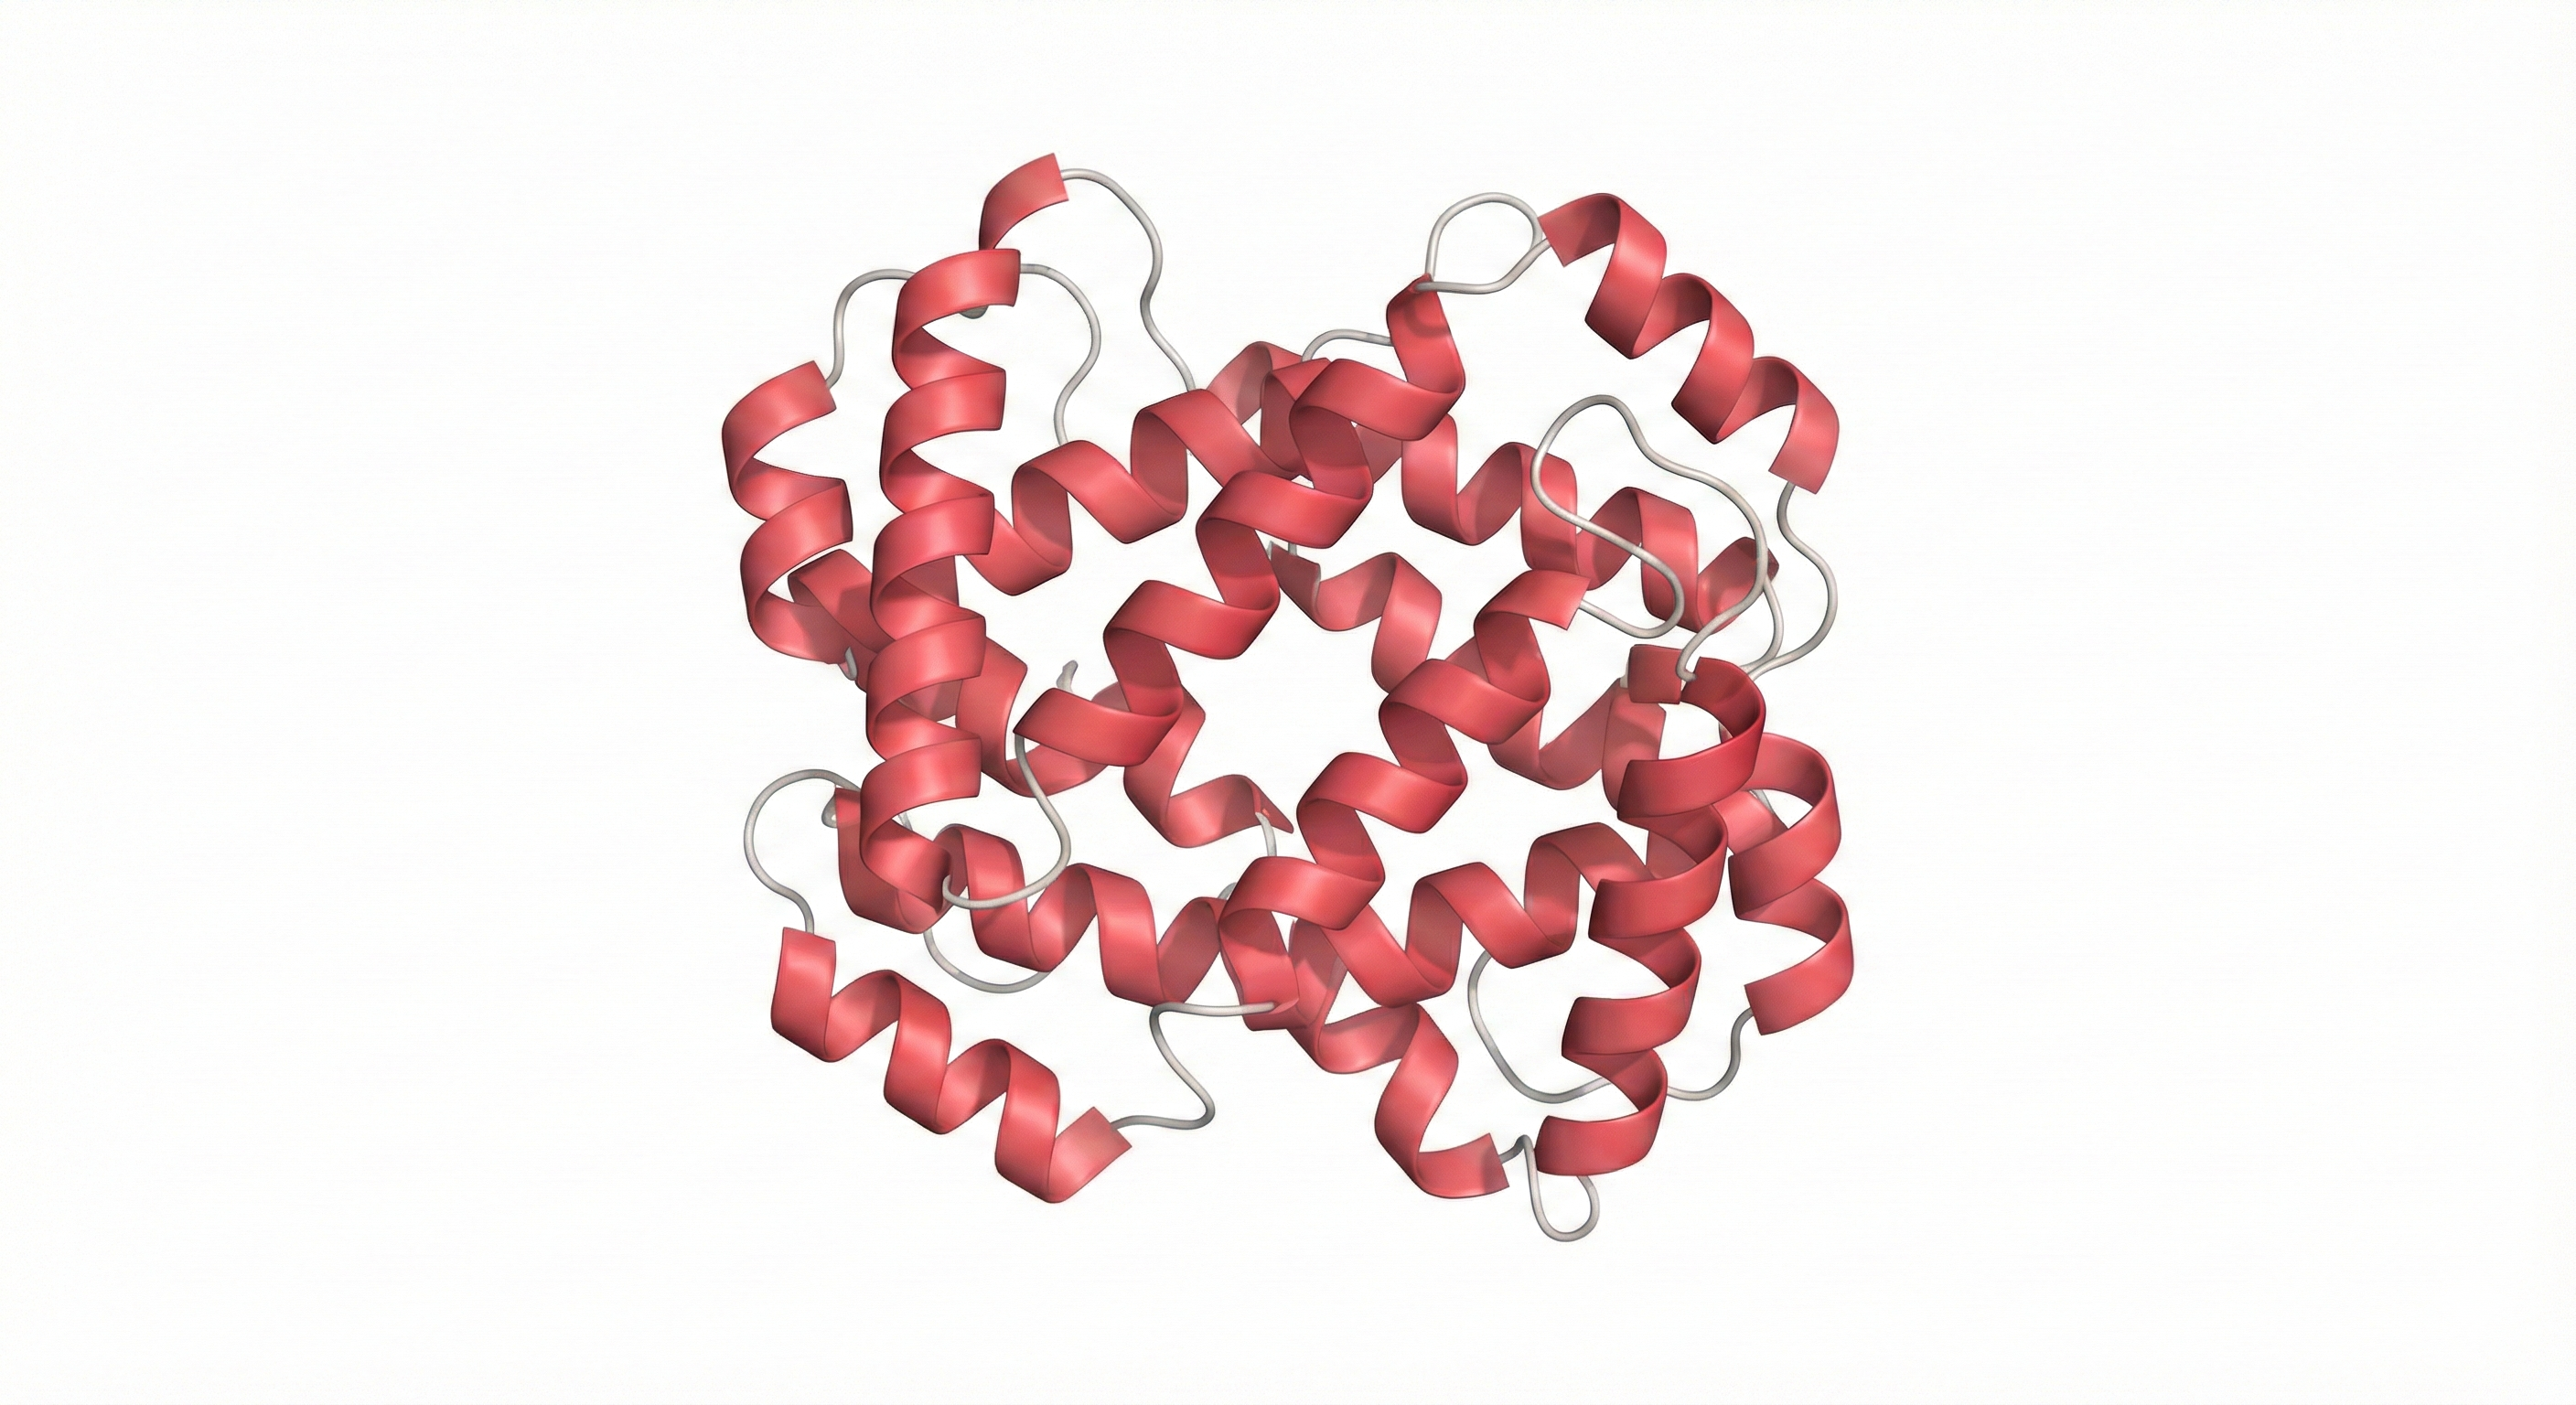
\includegraphics[width=0.5\textwidth]{Hemoglobin_subunit.png}
    \caption{Three-dimensional structure of the haemoglobin beta subunit - figure created by author using Nano Banana}
    \label{fig:hemoglobin}
\end{figure}

To make the problem more tractable, Dill introduced the Hydrophobic-Polar (HP) lattice model in 1985 \cite{Dill1985}. The model collapses the twenty amino acid types into two classes: hydrophobic residues (H), which tend to avoid water, and polar residues (P), which interact more favourably with it. A sequence is then embedded as a self-avoiding walk on a lattice, with each residue occupying a distinct site and successive residues constrained to lie on adjacent lattice points \cite{Lau1989}. Within this discrete setting, the objective is driven by hydrophobic contacts. The energy is defined by the number of non-consecutive H--H contacts, i.e., pairs of hydrophobic residues that are neighbours on the lattice but not adjacent along the chain. In effect, the optimisation target is to find an embedding that promotes hydrophobic clustering while respecting the self-avoidance and adjacency constraints.

Even under this simplified lattice formulation, HP folding remains computationally demanding. Crescenzi et al.\ proved in 1998 that the optimisation problem is NP-complete \cite{Crescenzi1998}, so one should not expect a method that scales efficiently across all instances as the sequence length increases. The practical consequences show up fairly quickly. By the time sequences are in the 30 to 50 residue range, the set of valid self-avoiding conformations is already large enough that exhaustive enumeration stops being a useful point of comparison. That is part of the reason the HP model is used so often in combinatorial optimisation research: it is clean to specify, hard to solve, and easy to evaluate consistently across algorithms.

Given that hardness, much of the earlier computational literature relied on heuristics rather than exact optimisation. Simulated annealing became a common choice from the 1990s onward because it provides a straightforward mechanism for escaping local minima by occasionally accepting unfavourable moves early in the search \cite{UngerMoult1993}. Genetic algorithms offered a different style of exploration, maintaining a population of candidate folds and gradually improving it through recombination and mutation operators \cite{Krasnogor2002Multimeme}. Tabu search was also explored, discouraging cycling by remembering recent states. Ant colony optimisation took yet another approach, biasing construction using information carried over from successful searches \cite{LeshPullMoves2003, StützleACO2005}.

Constraint programming (CP) offers an alternative to heuristic search for HP folding. Chain connectivity, self-avoidance, and contact formation can all be encoded directly as folding constraints and then pruned through propagation \cite{Barták2003}. Earlier CP tools, such as CPSP-tools, successfully tackled HP folding using specialised H-core databases and constraint satisfaction techniques \cite{CPSP2009}. Google OR-Tools CP-SAT extends this approach by combining it with SAT-style clause learning and linear programming relaxation \cite{Perron2023}. This can provide bounds on solution quality and, in favourable cases, certificates of optimality \cite{GoogleORTools}. Large Neighbourhood Search is also supported, allowing solutions to be improved iteratively \cite{Shaw1998}. Modern CP-SAT solvers, like CP-SAT, have not been applied to HP folding, as earlier CP tools were \cite{CPSP2009}, making this a fascinating venue worth revisiting.

While constraint programming guarantees optimality when feasible, its exponential scaling limits practical applicability to shorter sequences. Reinforcement learning has recently emerged as an alternative approach for HP folding. Espitia et al.\ (2024) applied Deep Q-learning to the three-dimensional HP model \cite{Espitia2024}. Folding was treated as a sequential decision problem, where agents can learn folding strategies through trial-and-error without explicitly encoding the problem constraints \cite{Yang2022}. Whether this reinforcement learning method can compete with exact solver approaches like CP-SAT remains unknown.

This study presents a comparison of constraint programming and reinforcement learning for the 3D HP protein folding problem. We implement a CP-SAT solver using Google OR-Tools, formulating the problem with one-hot encoding, chain adjacency constraints, and symmetry-breaking techniques. For the reinforcement learning comparison, we use the open-source LSTM-A (Long Short-Term Memory with multi-head Attention) Deep Q-Learning implementation from Espitia et al.\ (2024) \cite{Espitia2024}, training the model from scratch on our local machine. We evaluate both approaches on eight benchmark sequences (3d1--3d8) with lengths ranging from 20 to 58 residues to determine which method achieves better solution quality.

\textbf{Paper structure as follows:}
\begin{itemize}
    \item Chapter 2 describes the implementation and training procedures for each method.
    \item Chapter 3 presents comparative results and scaling behaviour.
    \item Chapter 4 discusses implications, limitations, and future directions.
\end{itemize}

\chapter{Methodology}

\section{Problem Formulation}

The HP protein folding problem on a three-dimensional lattice is defined as follows. A protein sequence is represented as a string:
\begin{equation}
S = s_1 s_2 \ldots s_n,
\end{equation}
where each residue $s_i$ is classified as either hydrophobic (H) or polar (P). A conformation $C$ is a self-avoiding walk on the three-dimensional integer lattice $\mathbb{Z}^3$, meaning each residue is placed at a distinct position:
\begin{equation}
c_i = (x_i, y_i, z_i) \in \mathbb{Z}^3,
\end{equation}
and no two residues occupy the same lattice point. The adjacency constraint requires that consecutive residues along the chain are placed at Manhattan distance 1:
\begin{equation}
||c_i - c_{i+1}||_1 = 1 \quad \forall i \in \{1, \ldots, n-1\}.
\end{equation}
where $||v||_1 = |x| + |y| + |z|$ for a vector $v = (x, y, z)$.

The energy of a conformation is determined by the number of non-consecutive H--H contacts. A contact occurs when two hydrophobic residues are neighbours on the lattice but not adjacent along the sequence. Formally, the energy function is defined as
\begin{equation}
E(C) = -\left|\{(i,j) : s_i = s_j = \text{H}, \, |i - j| > 1, \, ||c_i - c_j||_1 = 1\}\right|,
\end{equation}
where the set counts all pairs of non-consecutive H-residues that are lattice-adjacent. The objective is to minimise $E(C)$, which is equivalent to maximising the number of favourable hydrophobic contacts. This formulation reflects the simplified physical principle that hydrophobic residues prefer to cluster together, shielding themselves from the surrounding aqueous environment. An illustration of this energy function is provided in Figure~\ref{fig:hp_lattice}.

\begin{figure}[htbp]
    \centering
    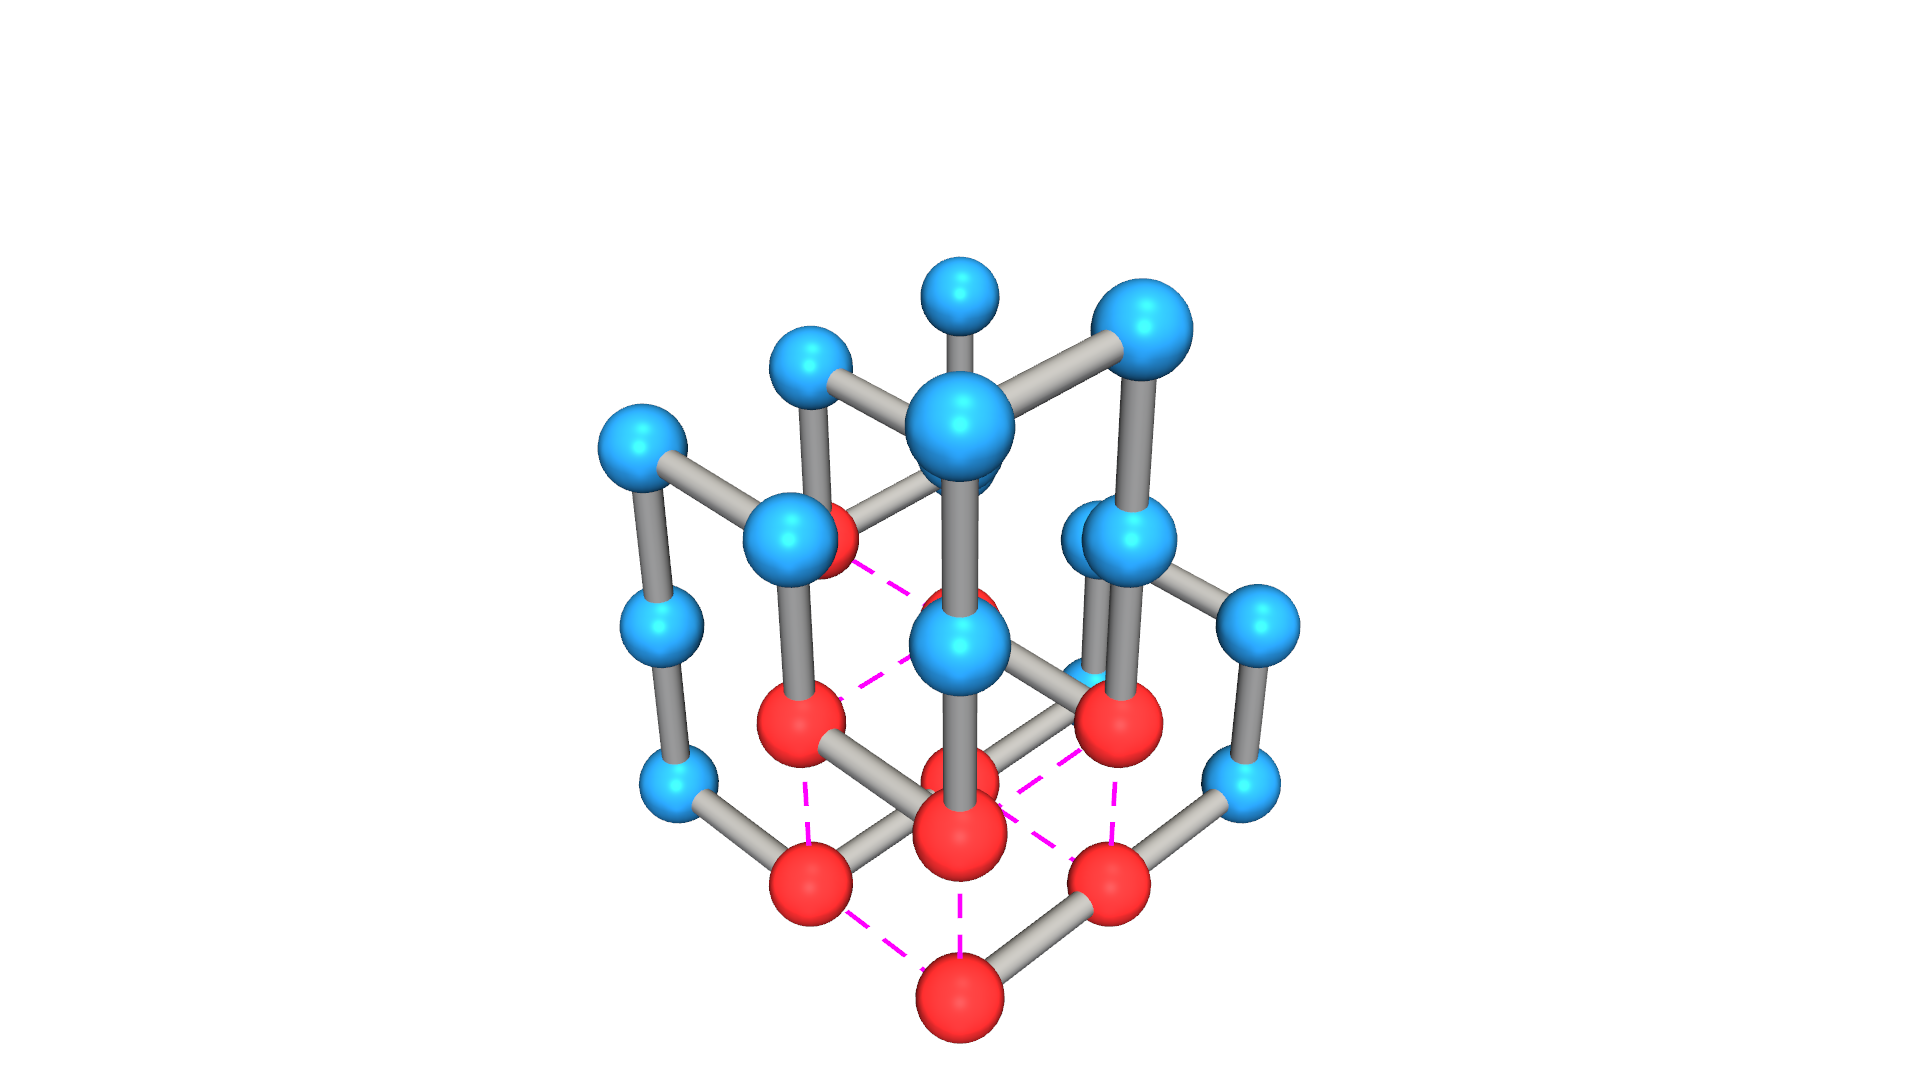
\includegraphics[width=0.6\textwidth]{3d3.png}
    \caption{Illustration of the 3D HP lattice model showing a short self-avoiding walk. Hydrophobic residues (H) are shown in red, polar residues (P) in blue. Dotted magenta lines indicate valid non-consecutive H--H contacts that contribute to the energy function, this contact has energy -9 $\epsilon_{HH}$.}
    \label{fig:hp_lattice}
\end{figure}

We evaluate both methods on a set of benchmark sequences drawn from the literature. Table~\ref{tab:benchmarks} lists the sequences used in this study, identified by their standard names (e.g., 3d1, 3d2, \ldots, 3d8). The sequences span a range of lengths from $n = 20$ to $n = 58$ residues and include both their H/P patterns and best-known energy values from prior work \cite{Espitia2024}.

\begin{table}[htbp]
\centering
\caption{Benchmark HP sequences used in this study. Best-known energies are taken from \cite{Espitia2024}.}
\label{tab:benchmarks}
\begin{tabular}{lc>{\centering\arraybackslash}p{6.8cm}c}
\toprule
\textbf{Seq.} & \textbf{Length} & \textbf{Sequence} & \textbf{Best-known Energy} \\
\midrule
3d1 & 20 & $(HP)^2PH(HP)^2(PH)^2HP(PH)^2$ & $-11$ \\
3d2 & 24 & $H^2P^2(HP^2)^6H^2$ & $-13$ \\
3d3 & 25 & $P^2HP^2(H^2P^4)^3H^2$ & $-9$ \\
3d4 & 36 & $P(P^2H^2)^2P^5H^5(H^2P^2)^2P^2H(HP^2)^2$ & $-18$ \\
3d5 & 46 & $P^2H^3PH^3P^3HPH^2PH^2P^2HPH^4$ \newline $PHP^2H^5PHPH^2P^2H^2P$ & $-35$ \\
3d6 & 48 & $P^2H(P^2H^2)^2P^5H^{10}P^6$ \newline $(H^2P^2)^2HP^2H^5$ & $-31$ \\
3d7 & 50 & $H^2(PH)^3PH^4PH(P^3H)^2P^4$ \newline $(HP^3)^2HPH^4(PH)^3PH^2$ & $-34$ \\
3d8 & 58 & $PH(PH^3)^2P(PH^2PH)^2H(HP)^3$ \newline $(H^2P^2H)^2PHP^4(H(P^2H)^2)^2$ & $-44$ \\
\bottomrule
\end{tabular}
\end{table}

\newpage{}

\section{CP-SAT Approach}
\label{sec:cpsat_approach}

This section describes our constraint programming implementation using Google OR-Tools CP-SAT solver~\cite{GoogleORTools, Perron2023}. We formulate the 3D HP folding problem as a constraint satisfaction problem, encoding the self-avoiding walk and contact constraints algebraically to maximise H--H contacts.

\subsection{Decision Variables}

Our CP-SAT formulation uses one-hot encoding to represent where residues sit on the 3D cubic lattice. In one-hot encoding, each position is indicated by a binary vector where exactly one element is set to 1 (indicating the residue occupies that position) and all others are 0. For each residue $i \in \{0, 1, \ldots, n-1\}$ and each cell $c = (x, y, z)$ in the grid:
\begin{equation}
\mathcal{G} = \{(x,y,z) : x,y,z \in \{0, 1, \ldots, L-1\}\},
\end{equation}
we create a binary decision variable:
\begin{equation}
x_{i,c} \in \{0, 1\},
\end{equation}
where $x_{i,c} = 1$ means residue $i$ occupies position $c$, and $x_{i,c} = 0$ otherwise. The grid dimension $L$ needs to provide enough space for sequences of length $n$, typically satisfying $L \geq \lceil n^{1/3} \rceil + 2$.

For each pair of non-consecutive hydrophobic residues $(i,j)$ with $|i-j| > 1$ and $S_i = S_j = \text{H}$, we introduce contact indicators:
\begin{equation}
c_{i,j} \in \{0, 1\},
\end{equation}
where $c_{i,j} = 1$ if residues $i$ and $j$ occupy adjacent cells at Manhattan distance 1, and $c_{i,j} = 0$ otherwise.

\subsection{Core Constraints}

The CP-SAT model enforces four main constraint types:

\paragraph{Placement constraint.} Each residue must sit in exactly one cell:
\begin{equation}
\sum_{c \in \mathcal{G}} x_{i,c} = 1 \quad \forall i \in \{0, \ldots, n-1\}.
\end{equation}

\paragraph{Self-avoidance constraint.} Each cell can hold at most one residue:
\begin{equation}
\sum_{i=0}^{n-1} x_{i,c} \leq 1 \quad \forall c \in \mathcal{G}.
\end{equation}

\paragraph{Adjacency constraint.} Consecutive residues in the sequence must occupy neighbouring cells on the lattice, creating the self-avoiding walk. For each consecutive pair $(i, i+1)$, if residue $i$ sits in cell $c$, then residue $i+1$ must occupy one of the six adjacent cells:
\begin{equation}
\mathcal{N}(c) = \{c' \in \mathcal{G} : \|c - c'\|_1 = 1\}.
\end{equation}
We encode this using logical implications:
\begin{equation}
x_{i,c} = 1 \implies \sum_{c' \in \mathcal{N}(c)} x_{i+1,c'} = 1 \quad \forall i \in \{0, \ldots, n-2\}, \, \forall c \in \mathcal{G}.
\end{equation}

\paragraph{Contact linking constraint.} The contact indicators $c_{i,j}$ are linked to placement variables through reified constraints (constraints represented as boolean variables that can be true or false) that ensure $c_{i,j} = 1$ exactly when residues $i$ and $j$ occupy adjacent cells, while excluding consecutive backbone edges.

\subsection{Symmetry Breaking}

The cubic lattice has 48 symmetries from rotations and reflections. To cut down the search space and speed up solving, we fix the first two residues at the grid center:
\begin{align}
x_{0, (\lfloor L/2 \rfloor, \lfloor L/2 \rfloor, \lfloor L/2 \rfloor)} &= 1, \\
x_{1, (\lfloor L/2 \rfloor, \lfloor L/2 \rfloor, \lfloor L/2 \rfloor - 1)} &= 1.
\end{align}
This pins residue 0 at the center and residue 1 along the negative $z$-axis, which canonicalises the representation by providing a unique representative conformation from each equivalence class of symmetry-related solutions. This approach shrinks the search space by a factor of 48 without losing any optimal solutions.

\subsection{Objective Function}

The goal is to maximise the total number of non-consecutive H--H contacts. Let $\mathcal{H} = \{i : s_i = \text{H}\}$ denote the set of hydrophobic residue indices. The objective is:
\begin{equation}
\text{maximise} \quad \sum_{(i,j) \in \mathcal{C}} c_{i,j},
\end{equation}
where $\mathcal{C} = \{(i,j) : i,j \in \mathcal{H}, \, i < j, \, |i - j| > 1\}$ is the set of potential non-consecutive H--H contact pairs. Since the energy function is $E(C) = -\varepsilon_{HH} \cdot \sum_{(i,j) \in \mathcal{C}} c_{i,j}$, maximising contacts is equivalent to minimising energy.

\subsection{Solver Configuration}

We use Google OR-Tools CP-SAT version 9.11 with this setup for each sequence:
\begin{itemize}
\item \textbf{Optimisation phase:} 560 seconds (20\% of time budget) for finding the best grid size and tuning parameters across 5 random seeds
\item \textbf{Final solve phase:} 2240 seconds (80\% of time budget) with optimised settings
\item \textbf{Parallelisation:} 8 worker threads running parallel search
\item \textbf{Total time budget:} 2800 seconds (roughly 47 minutes per sequence)
\end{itemize}
We determine grid size $L$ during the optimisation phase by testing values from $\lceil n^{1/3} \rceil + 2$ up to this value plus 3, picking the smallest grid that gives good solutions. The solver uses branch-and-bound search (a divide-and-conquer method that recursively splits the solution space while pruning branches proven suboptimal) with constraint propagation, conflict-driven clause learning, and automatic search strategies. When the solver finishes with \texttt{OPTIMAL} status, the solution is provably the best possible. When it stops with \texttt{FEASIBLE} status, the solution is valid but we can't guarantee it's optimal.
\newpage{}

\section{LSTM-A Deep Q-Learning Approach}
\label{sec:lstma_approach}

This section describes the LSTM-A (Long Short-Term Memory with multi-head Attention) architecture from Espitia et al.\ (2024) \cite{Espitia2024}, a deep reinforcement learning approach that combines recurrent neural networks with attention mechanisms for protein folding. The method uses Deep Q-Learning to train an agent that learns to place residues sequentially on the 3D lattice, maximising H--H contacts through trial-and-error interaction with the environment. Unlike purely feedforward or transformer-based Q-networks, LSTM-A processes the folding trajectory autoregressively using LSTM hidden states to maintain memory of the partial conformation, while multi-head attention layers enable the model to attend to all previously placed residues when selecting the next placement action. We use their publicly available implementation, training models from scratch on our local machine for each benchmark sequence.

\subsection{Markov Decision Process Formulation}

The 3D HP folding problem is formulated as a Markov Decision Process (MDP) defined by the tuple $(\mathcal{S}, \mathcal{A}, P, R, \gamma)$.

The \textbf{state space} $\mathcal{S}$ consists of one-hot encoded vectors representing the folding trajectory. Each state is represented as a tensor of shape $(n, 8, 1)$, where $n$ is the sequence length. At each position in the sequence, the 8-dimensional vector encodes:
\begin{equation}
s_i = [\text{ND}, \text{F}, \text{L}, \text{R}, \text{U}, \text{D}, \text{H}, \text{P}],
\end{equation}
where the first six elements represent the available actions (No Decision, Forward, Left, Right, Up, Down) and the last two elements indicate the amino acid type (Hydrophobic or Polar). Importantly, the network does not directly observe 3D coordinates; instead, it infers spatial configurations from the sequence of actions taken.

The \textbf{action space} $\mathcal{A}$ consists of five discrete relative placement directions:
\begin{equation}
\mathcal{A} = \{\text{Forward}, \text{Left}, \text{Right}, \text{Up}, \text{Down}\}.
\end{equation}
Each action specifies where to place the next residue relative to the current chain orientation. Backward moves are excluded since backtracking would violate the self-avoiding walk constraint.

The \textbf{transition dynamics} are deterministic:
\begin{equation}
P(s_{t+1} | s_t, a_t) : \text{deterministic},
\end{equation}
where action $a_t$ determines the placement of the next residue based on the current chain orientation. Episodes terminate successfully when all $n$ residues are placed without collision, or terminate early if the agent reaches a configuration where no valid placements remain.

The \textbf{reward function} $R(s_t, a_t)$ is sparse, providing feedback only upon episode termination:
\begin{equation}
R(s_t, a_t) = 
\begin{cases}
\sum_{(i,j)} c_{i,j} & \text{if all residues placed successfully} \\
0 & \text{otherwise}
\end{cases},
\end{equation}
where $c_{i,j} = 1$ indicates a valid H--H contact between non-consecutive hydrophobic residues $i$ and $j$ at Manhattan distance 1. This reward equals the negative energy $-E(C)$ from the problem formulation.

\subsection{Environment Implementation}

Espitia et al.'s implementation uses a custom Gymnasium environment with the following features:

\paragraph{Bounded coordinate system.} Residue positions are constrained to lie within a cubic bounding box:
\begin{equation}
[-r, r]^3 \quad \text{where} \quad r = \lfloor n/2 \rfloor.
\end{equation}
This prevents unbounded exploration and focuses search on compact conformations.

\paragraph{Symmetry breaking.} To reduce the search space by a factor of 48 (24 rotational symmetries $\times$ 2 reflections), the environment enforces two constraints: the first non-forward turn must be to the right, and the first vertical deviation must be upward. This canonicalises equivalent conformations under lattice symmetries, providing a unique representative from each symmetry class.

\paragraph{Trap detection.} The environment identifies dead-end configurations where no valid actions remain for the next residue placement. When trapped, the episode terminates immediately with zero reward, providing an implicit penalty that discourages exploration of unproductive regions.

\paragraph{Action masking.} At each step, the environment computes a boolean mask:
\begin{equation}
m \in \{0,1\}^{|\mathcal{A}|},
\end{equation}
indicating which actions satisfy three criteria: they do not violate the bounded region, they do not cause collisions with existing residues, and they do not lead immediately to a trapped state. This mask is used during action selection to restrict the agent's choices to feasible actions only.

\subsection{LSTM-A Network Architecture}

The action-value function $Q(s,a)$ uses the LSTM-A architecture from Espitia et al.\ \cite{Espitia2024}, which combines Long Short-Term Memory networks with multi-head attention. The architecture processes the $(n, 8, 1)$ state tensor representing one-hot encoded actions and amino acid types:

\paragraph{LSTM layer.} The input tensor is processed through an LSTM layer with hidden size $d = 512$. The LSTM maintains hidden states that capture sequential dependencies in the folding trajectory, processing each timestep's 8-dimensional one-hot vector sequentially.

\paragraph{Multi-head attention.} The LSTM outputs at all positions are refined using a multi-head self-attention mechanism with 4 heads. Given the LSTM hidden states $H \in \mathbb{R}^{n \times 512}$, each attention head computes:
\begin{equation}
\text{Attention}_i(Q, K, V) = \text{softmax}\left(\frac{QK^T}{\sqrt{d_k}}\right)V,
\end{equation}
where $Q$, $K$, and $V$ are linear projections of the LSTM output $H$, and $d_k$ is the dimension of the key vectors. The softmax function converts a vector of real numbers into a probability distribution:
\begin{equation}
\text{softmax}(\mathbf{z})_j = \frac{\exp(z_j)}{\sum_{k=1}^{n} \exp(z_k)},
\end{equation}
where $\mathbf{z} = [z_1, \ldots, z_n]$ is the input vector. The output is a vector of positive values that sum to 1, which ensures attention weights form a valid probability distribution. The outputs from all heads are concatenated and projected:
\begin{equation}
\text{MultiHead}(H) = \text{Concat}(\text{head}_1, \ldots, \text{head}_4)W^O.
\end{equation}
This allows the model to attend to all previously placed residues when evaluating the next action, enabling it to capture both local sequential patterns and long-range dependencies in the protein structure.

\paragraph{Output layer.} The final output is obtained by selecting the last timestep of the attention output, followed by a fully connected layer that maps to Q-values for the 5 placement actions.

\begin{figure}[htbp]
    \centering
    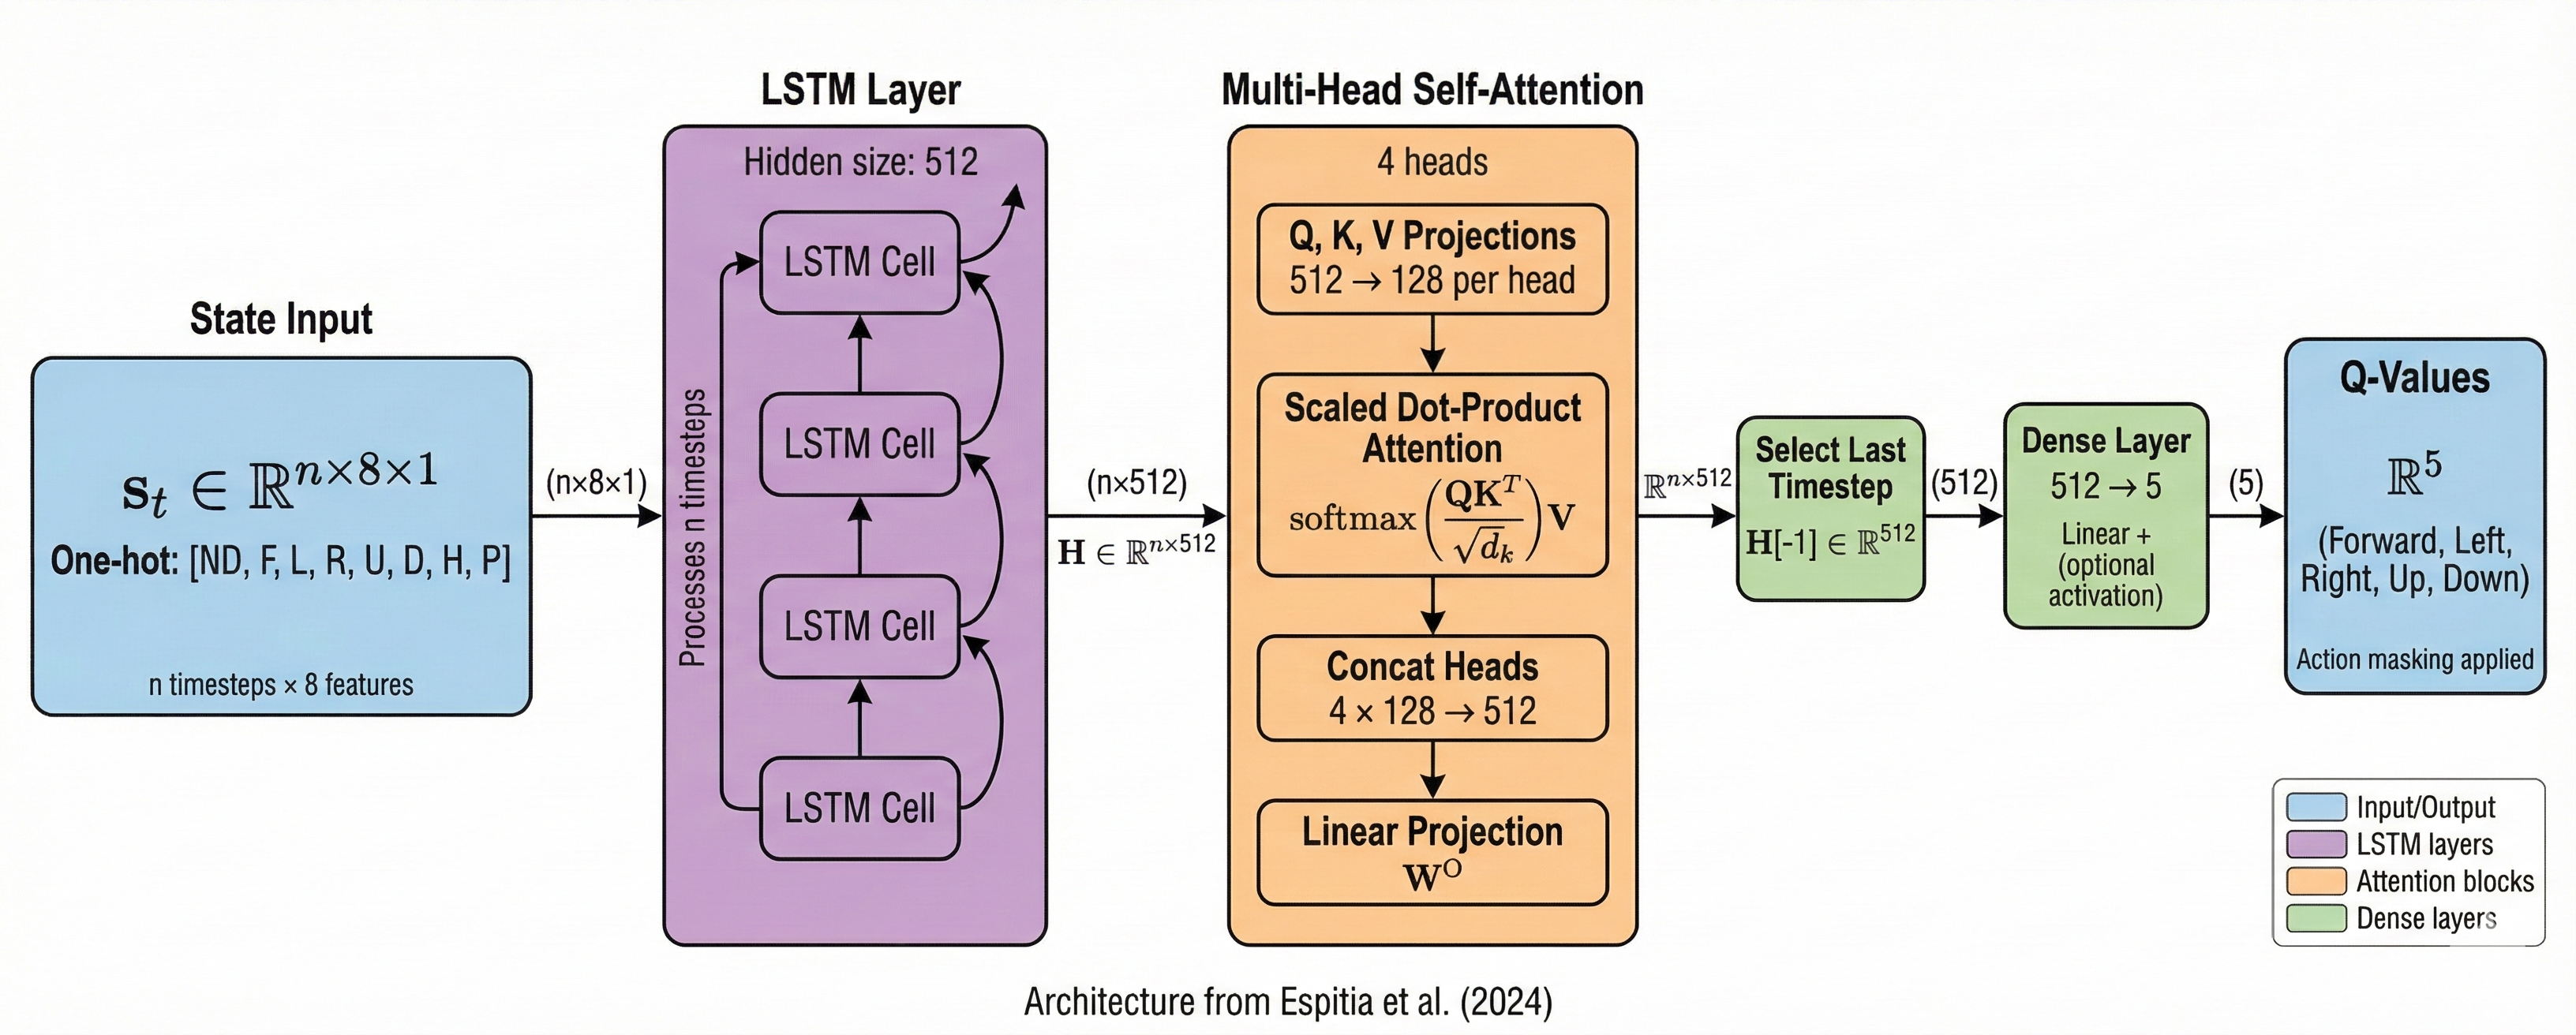
\includegraphics[width=0.95\textwidth]{fig_dqn_architecture.png}
    \caption{LSTM-A architecture from Espitia et al.\ (2024). The state input $(n, 8, 1)$ is processed through LSTM cells (hidden size 512) followed by 4-head multi-head self-attention. The last timestep of the attention output is mapped to Q-values for the 5 placement actions through a dense layer. Figure created by the author using Nano Banana.}
    \label{fig:dqn_architecture}
\end{figure}

\subsection{Training Protocol}

Espitia et al.'s training procedure uses Deep Q-Learning with several stabilisation techniques:

\paragraph{Double DQN.} To mitigate overestimation bias, two networks are maintained: a policy network $Q(s,a; \theta)$ and a target network $Q(s,a; \theta^-)$. The policy network selects actions during target computation, while the target network evaluates them:
\begin{equation}
y_t = r_t + \gamma \, Q(s_{t+1}, \arg\max_{a'} Q(s_{t+1}, a'; \theta) ; \theta^-).
\end{equation}
The target network parameters $\theta^-$ are updated by copying from the policy network every 1000 training steps.

\paragraph{Prioritised experience replay.} Transitions $(s_t, a_t, r_t, s_{t+1}, d_t)$ are stored in a replay \\buffer.
Transitions are sampled with probability proportional to their temporal-difference error:
\begin{align}
p_t &\propto |\delta_t|^\alpha \quad \text{where} \\
\delta_t &= y_t - Q(s_t, a_t; \theta) \quad \text{and} \quad \alpha = 0.6,
\end{align}
where $\delta_t$ is the TD error and $\alpha$ controls prioritisation strength. Since high-priority transitions are sampled more frequently, they would be overrepresented in gradient updates without correction. Importance sampling weights address this bias:
\begin{equation}
w_t = (N \cdot p_t)^{-\beta},
\end{equation}
where $N$ is the replay buffer size, $p_t$ is the sampling probability of transition $t$, and $\beta$ anneals from 0.4 to 1.0 during training to gradually increase the bias correction.

\paragraph{Action masking with $\varepsilon$-greedy exploration.} During training, actions are selected using an $\varepsilon$-greedy policy restricted to valid actions. With probability $\varepsilon$, the agent selects uniformly from the set of valid actions indicated by the environment's action mask. Otherwise, it selects:
\begin{equation}
\arg\max_{a \in \mathcal{A}_{\text{valid}}} Q(s,a;\theta),
\end{equation}
where invalid actions have their Q-values set to $-10^9$ to prevent selection. The exploration rate decays exponentially:
\begin{equation}
\varepsilon_t = \max(0.01, 1.0 \cdot 0.9995^t).
\end{equation}

\paragraph{Hyperparameters and training details.} Following Espitia et al., separate models are trained for each benchmark sequence. Table~\ref{tab:lstm_hyperparameters} summarises the training configuration.

\begin{table}[htbp]
\centering
\caption{LSTM-A training hyperparameters from Espitia et al.\ (2024)}
\label{tab:lstm_hyperparameters}
\begin{tabular}{ll}
\toprule
\textbf{Parameter} & \textbf{Value} \\
\midrule
\multicolumn{2}{l}{\textit{Network Architecture}} \\
LSTM hidden size & 512 \\
Attention heads & 4 \\
\midrule
\multicolumn{2}{l}{\textit{Training Configuration}} \\
Optimiser & Adam \\
Learning rate & $1.0 \times 10^{-3}$ \\
Discount factor $\gamma$ & 0.98 \\
Batch size & 16 (short seq.), 32 (long seq.) \\
Training episodes & 200K--250K (short), 500K--750K (long) \\
\midrule
\multicolumn{2}{l}{\textit{Stabilisation Techniques}} \\
Target network update & Every 1,000 steps \\
PER $\alpha$ (prioritisation) & 0.6 \\
PER $\beta$ (importance sampling) & 0.4 $\to$ 1.0 (annealed) \\
$\varepsilon$-greedy decay & $\max(0.01, 1.0 \cdot 0.9995^t)$ \\
\bottomrule
\end{tabular}
\end{table}

\chapter{Experiments and Results}
\label{chap:results}

\section{Experimental Setup}

All experiments were conducted on an Apple MacBook Pro with M2 Max chip and 32 GB unified memory. The CP-SAT solver was implemented using Google OR-Tools version 9.11, while the LSTM-A DQN implementation was obtained from Espitia et al.\ (2024) \cite{Espitia2024} and executed locally. Both methods were evaluated on the standard 3D HP benchmark sequences (3d1--3d8) published by \cite{Espitia2024}, with best-known energy values serving as optimality targets.

\subsection{CP-SAT Experiments}

For CP-SAT, we allocated a total computational budget of 7 hours distributed across all 8 sequences (3d1--3d8), yielding approximately 47 minutes per sequence. Each sequence underwent a two-phase optimisation: 20\% of the budget (9 minutes, 20 seconds) for grid size exploration and parameter tuning across 5 random seeds, and 80\% of the budget (37 minutes, 20 seconds) for final optimisation with the best-discovered settings. The solver used 8 parallel worker threads throughout. All CP-SAT results reported in this chapter were obtained from our own experimental runs.

\subsection{LSTM-A DQN Experiments}

For the LSTM-A agent, we attempted to replicate the training protocol described in Section~\ref{sec:lstma_approach} on our local machine. However, due to the substantial computational requirements and extended training times on CPU (the M2 Max lacks CUDA support for PyTorch), we were only able to complete training runs for sequences 3d1 and 3d2. 

Given these resource constraints, we report a combination of results: our locally obtained results for 3d1 and 3d2, supplemented by the published results from Espitia et al.\ (2024) for sequences 3d3--3d8. Figure~\ref{fig:training_curves} shows representative training dynamics from Espitia et al.\ for sequences of varying lengths, illustrating how training complexity scales with sequence size.

\begin{figure}[p]
    \centering    
    \begin{subfigure}[t]{0.75\textwidth}
        \centering
        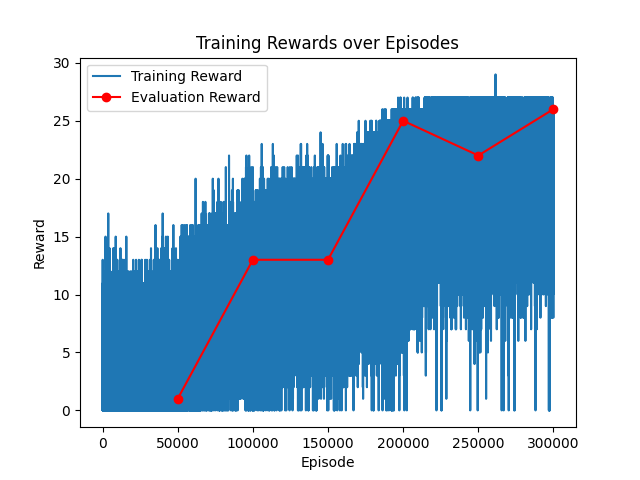
\includegraphics[width=\textwidth]{training_rewards_48.png}
        \caption{Length 48 (3d6)}
        \label{fig:training_48}
    \end{subfigure}
    
    % \vspace{1.5em}
    
    \begin{subfigure}[t]{0.75\textwidth}
        \centering
        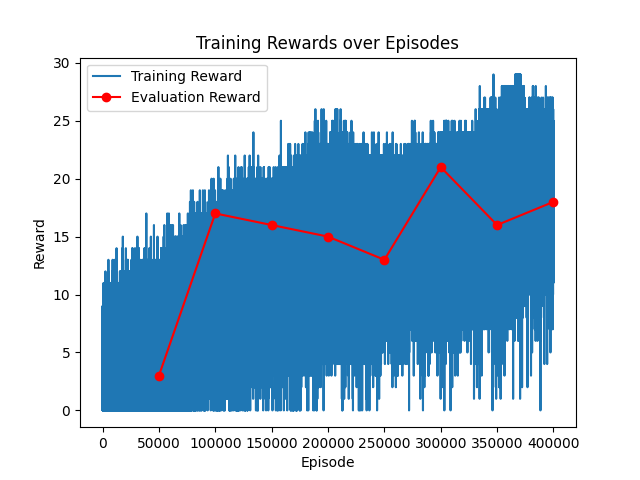
\includegraphics[width=\textwidth]{training_rewards_50.png}
        \caption{Length 50 (3d7)}
        \label{fig:training_50}
    \end{subfigure}
    \caption{LSTM-A training convergence curves from Espitia et al.\ (2024) for sequences of varying lengths. Blue areas show training rewards, red lines show evaluation performance.}
    \label{fig:training_curves}
\end{figure}

All results tables in this chapter clearly indicate the source of each result, distinguishing between our experimental runs and values taken from the original paper.
\newpage{}

\section{Solution Quality and Comparative Analysis}

Table~\ref{tab:benchmark_results} presents the energy values achieved by both methods on the 3D HP benchmark sequences. The energy is defined as the negative count of non-consecutive H--H contacts, so more negative values indicate better (more stable) conformations.

\begin{table}[htbp]
\centering
\caption{Solution quality on 3D HP benchmark sequences. Energy is the negative count of H--H contacts; lower (more negative) values are better. All CP-SAT results from our experiments; LSTM-A results: \textsuperscript{†}our local runs, others from Espitia et al.\ (2024).}
\label{tab:benchmark_results}
\begin{tabular}{lrrrr}
\toprule
\textbf{Seq.} & \textbf{Len} & \textbf{CP-SAT} & \textbf{LSTM-A} & \textbf{Best Known}\\
\midrule
3d1 & 20 & $-11$ & $-11$\textsuperscript{†} & $-11$ \\
3d2 & 24 & $-13$ & $-13$\textsuperscript{†} & $-13$ \\
3d3 & 25 & $-9$  & $-9$  & $-9$  \\
3d4 & 36 & $-18$ & $-18$ & $-18$ \\
3d5 & 46 & $-32$ & $-33$ & $-35$ \\
3d6 & 48 & $-29$ & $-30$ & $-31$ \\
3d7 & 50 & $-30$ & $-29$ & $-34$ \\
3d8 & 58 & $-40$ & $-40$ & $-44$ \\
\bottomrule
\end{tabular}
\end{table}

Both methods demonstrate strong performance on shorter sequences (3d1--3d4, lengths 20--36), matching the best-known energy values exactly. The CP-SAT solver terminated with \texttt{OPTIMAL} status for these sequences, providing certificates of optimality through exhaustive branch-and-bound search within the allocated time budget. Based on our local runs for 3d1--3d2 and published results from Espitia et al.\ for 3d3--3d8, the LSTM-A agent matched these optimal values through learned sequential placement policies, successfully recognising and exploiting hydrophobic clustering patterns via its LSTM-attention architecture.

On longer sequences (3d5--3d8, lengths 46--58), neither method reaches the best-known values. CP-SAT maintains gaps of 2--4 contacts from the literature values, unable to prove optimality within the time limit as the exponential search space growth overwhelms the constraint propagation and symmetry-breaking techniques. LSTM-A shows similar performance with gaps of 2--5 contacts: achieving $-33$ on 3d5 (within 2 of best-known), $-30$ on 3d6 (within 1), $-29$ on 3d7 (5 away), and $-40$ on 3d8. Notably, both methods converge to identical energy values on the longest sequence 3d8 (length 58), suggesting they face similar fundamental challenges in scaling to longer sequences.

Figure~\ref{fig:quality_vs_length} visualises these results, clearly showing the transition from optimal performance on shorter sequences to increasing gaps on longer ones.

\begin{figure}[htbp]
    \centering
    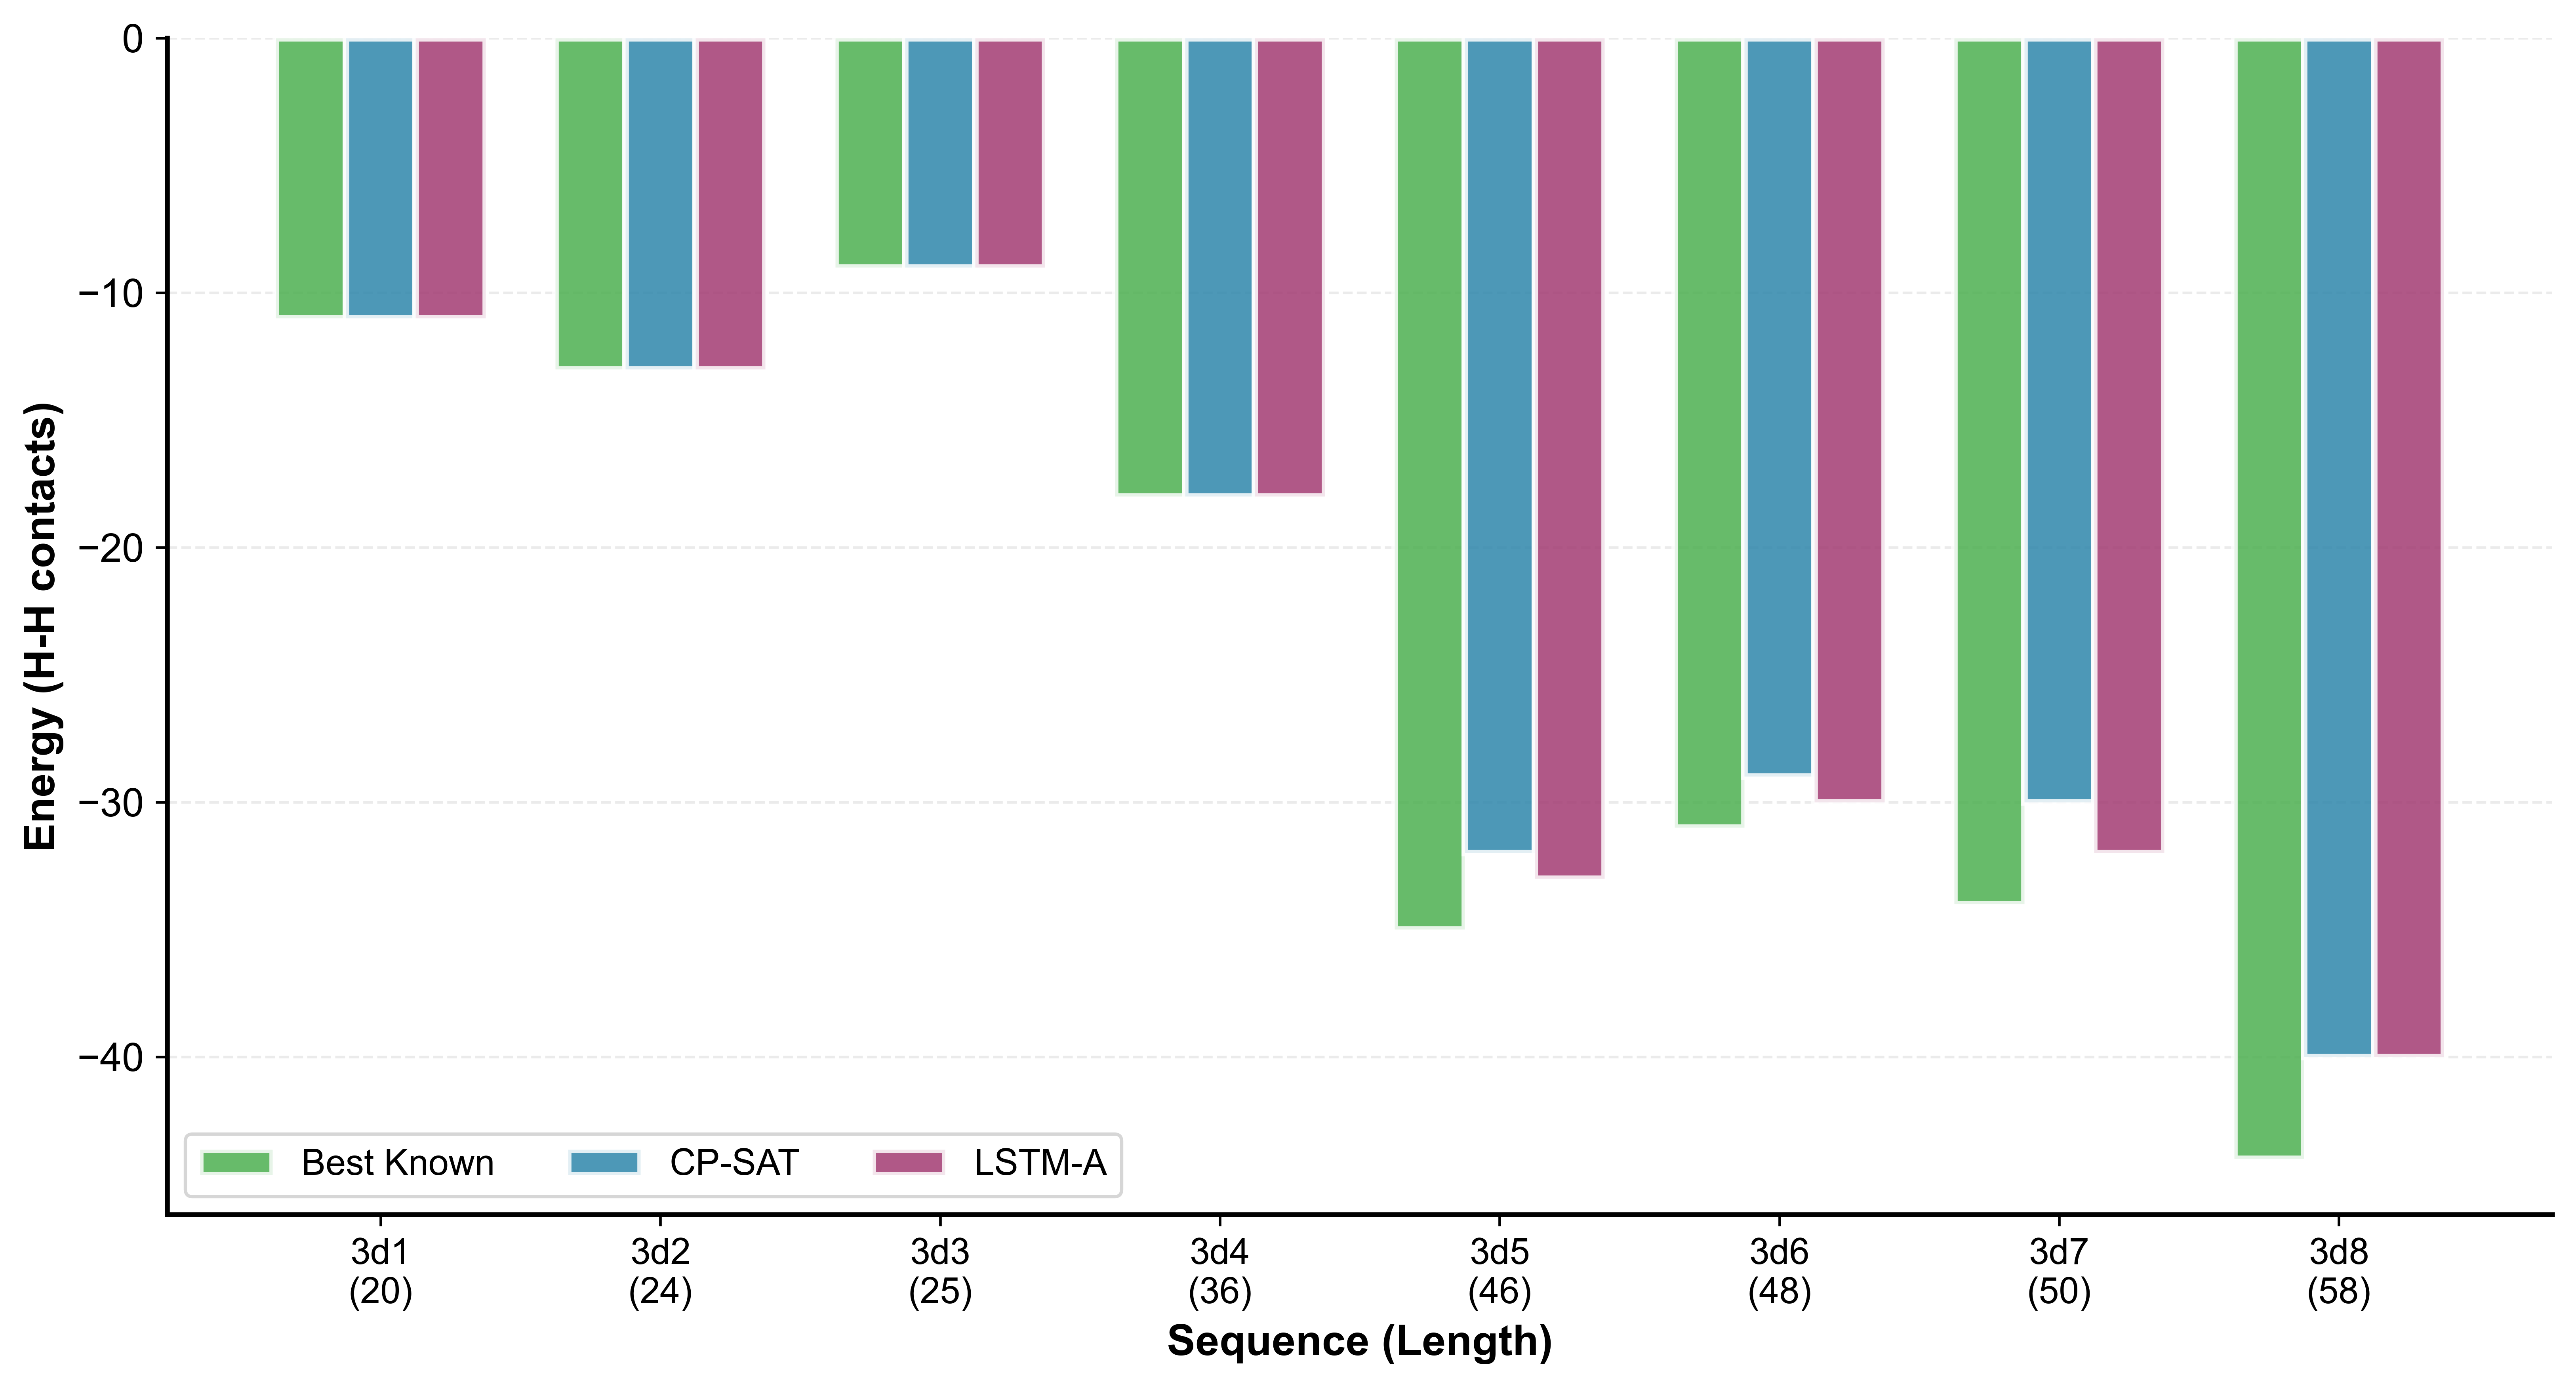
\includegraphics[width=0.9\textwidth]{fig_energy_comparison.png}
    \caption{Solution quality comparison across benchmark sequences. Both methods achieve optimal solutions for sequences up to length 36 (3d1--3d4). Performance degrades gracefully on longer sequences, with gaps of 2--5 contacts from best-known values.}
    \label{fig:quality_vs_length}
\end{figure}

Figure~\ref{fig:3d7_comparison} illustrates representative conformations for sequence 3d7 (length 50), where CP-SAT achieved $-30$ contacts compared to LSTM-A's $-29$ contacts, demonstrating the one-contact advantage of systematic constraint-based search on this instance.

\begin{figure}[p]
    \centering
    \begin{subfigure}[t]{0.85\textwidth}
        \centering
        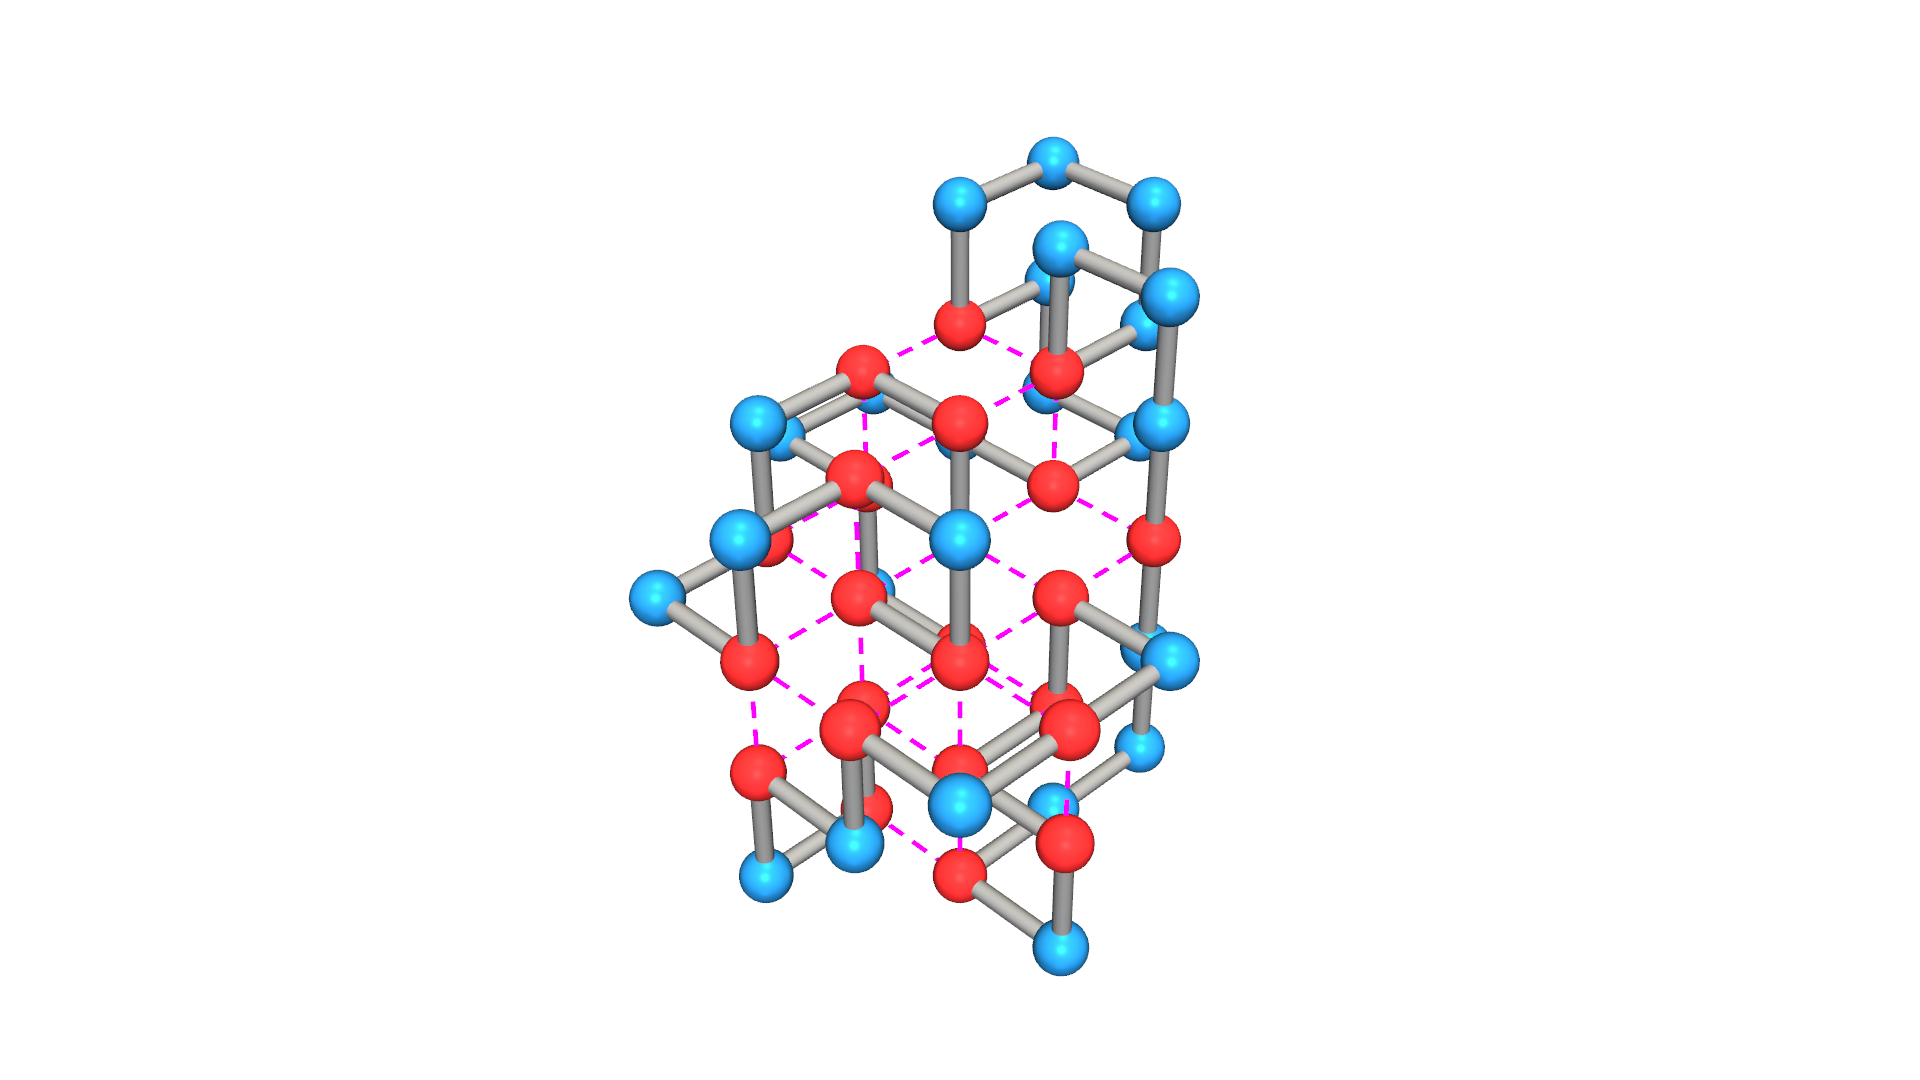
\includegraphics[width=\textwidth]{3d7_cpsat.png}
        \caption{CP-SAT solution: Energy = $-30$ contacts}
        \label{fig:3d7_cpsat}
    \end{subfigure}
    
    \vspace{1.5em}
    
    \begin{subfigure}[t]{0.85\textwidth}
        \centering
        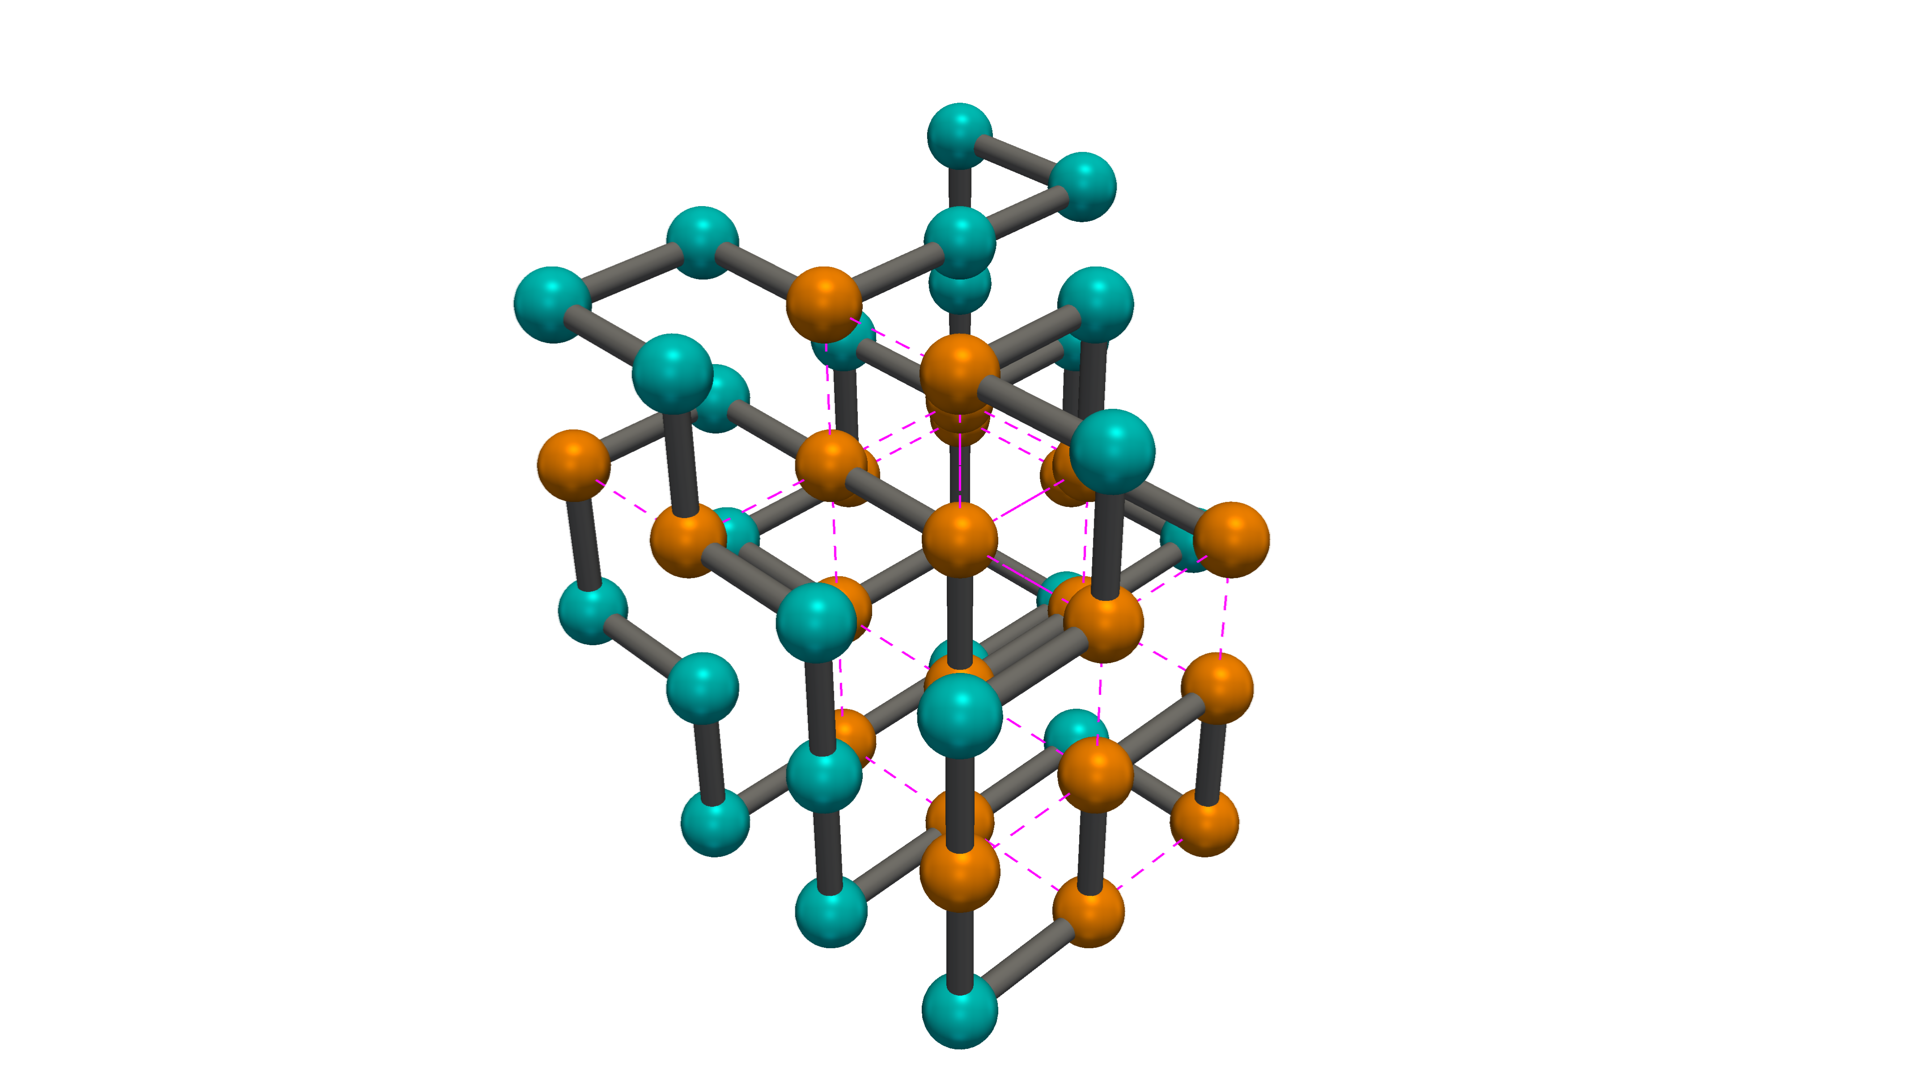
\includegraphics[width=\textwidth]{3d7_lstma.png}
        \caption{LSTM-A solution: Energy = $-29$ contacts}
        \label{fig:3d7_lstma}
    \end{subfigure}
    \caption{Conformations for sequence 3d7 (length 50). (a) CP-SAT achieves $-30$ contacts (red = H, blue = P). (b) LSTM-A achieves $-29$ contacts (orange = H, cyan = P). Magenta lines mark non-consecutive H--H contacts.}
    \label{fig:3d7_comparison}
\end{figure}

\chapter{Discussion}
\label{chap:discussion}

This study compared constraint programming (CP-SAT) against reinforcement learning (LSTM-A) for the 3D HP protein folding problem, addressing whether systematic search with guarantees or learning-based exploration better handles this NP-hard combinatorial optimisation task.

Both methods achieved identical results on sequences up to length 36, with CP-SAT providing optimality certificates through exhaustive search and LSTM-A discovering the same conformations through learned policies. This demonstrates that reinforcement learning can match exact optimisation quality when the problem remains tractable. The LSTM-attention architecture successfully captured geometric patterns for maximising hydrophobic contacts, validating that neural networks can learn the structure of protein conformational landscapes. Performance diverged on longer sequences (46--58 residues), where both methods fell 2--5 contacts short of best-known values. CP-SAT's gaps reflect exponential search space growth overwhelming constraint propagation, while LSTM-A's gaps suggest learned policies struggle to generalise beyond training distributions. Their convergence to identical energies on the longest sequence (3d8: both achieving $-40$) indicates they encounter similar local optima despite completely different search strategies.

CP-SAT provides optimality guarantees when tractable, making it ideal for benchmarking and establishing ground truth. The solver's deterministic behaviour ensures reproducibility and enables rigorous analysis through statistics. However, NP-hardness fundamentally limits scalability. Even sophisticated pruning eventually fails as search space grows exponentially. LSTM-A learns generalisable placement policies from experience, potentially enabling faster solutions on similar sequences through transfer learning. The architecture naturally models both sequential dependencies (LSTM) and long-range relationships (attention). Our replication of published 3d1--3d2 results confirms reproducibility, though computational constraints prevented validation on longer sequences. 

Computational constraints limited our LSTM-A validation to sequences 3d1--3d2, with longer sequences using published results from Espitia et al. While successful replication confirms reproducibility, independent verification would strengthen conclusions. Fixed CP-SAT time budgets (47 minutes per sequence) may not reflect true asymptotic performance, and we adopted published LSTM-A hyperparameters without extensive per-sequence tuning.

Future work should explore hybrid approaches combining CP-SAT's optimality-seeking with LSTM-A's pattern recognition. For example, using CP-SAT to generate diverse training data or learned policies to warm-start branch-and-bound search. Transfer learning deserves investigation: can models pretrained on shorter sequences accelerate longer ones? Do models transfer across sequences with similar hydrophobic patterns?

\section*{Code Availability}

The software, code, and data used in this study are available in public GitHub repositories and Github Gists:

\begin{itemize}
    \item \textbf{CP-SAT Implementation:} \url{https://github.com/pranav-ramanathan/HP-CSP}
    \item \textbf{LSTM-A DQN Implementation:} \url{https://github.com/AnonymousAuthor117/Protein-Structure-Prediction-in-the-3D-HP-Model-Using-Deep-Reinforcement-Learning}
    \item \textbf{Image Generation Prompts:} \url{https://gist.github.com/pranav-ramanathan/f5a4f8effa07861ef452e802132e2dc8}
\end{itemize}


\bibliographystyle{unsrtnat}
\bibliography{references}  

\end{document}